\documentclass[12pt]{article}
\usepackage{graphicx}
\usepackage{hyperref}
\title{Testing Policy}
\author{Binary Ninjaz}
\date{}
\begin{document}
  \maketitle

\begin{flushright} \large

\includegraphics[width=30px]{leaf2}\emph{} \newline\newline 
Teboho Mokoena \emph{14415888} \newline
Sizo Duma \emph{15245579} \newline
Shaun Yates 	\emph{16007493} \newline
Letanyan Arumugam \emph{14228123} \newline
Kevin Reid\emph{15008739} \newline
John Ojo \emph{15096794} \newline
\end{flushright}
  \newpage
  
  \tableofcontents
  \newpage
  
  \section{INTRODUCTION}
  This document details the policies that BinaryNinjaz will be using to guide development and ensure a quality product. We describe why we intend to use specific testing methods and how their effects will impactful in our process. 
  
  \section{PURPOSE}
  Automated testing is vital and ensuring that the number of bugs in a program is as limited as possible. While having automated testing does not guarantee there will be no bugs in a program it can greatly reduce any bugs from appearing when you might not expect them to. While we intend to have a comprehensive test suite, we will not accept that wholly passing test cases mean that a program is without flaw.

\section{WHY IS TESTING REQUIRED?}
Testing forms an essential precondition to ensure the successful construction and implementation of information systems. The complexity of modern-day software is such that it is almost impossible to implement it correctly the first time around, without any form of verification.\newline\newline Testing is needed in order to detect potential problems within the software as early as possible, so that they can be corrected at minimum cost.\newline\newline  A second reason to carry out tests is to develop trust in and a knowledge of the product provided.\newline\newline Defects that exist within a software product can have severe consequences for the “business” and the users alike.  Whilst providing a means of avoiding faults as much as possible, testing is also a useful way of demonstrating to management and users that the product supplied fulfils their requirements (is “fit for purpose”).\newline\newline It is important to note in this regard that both the functionality and the non-functional software characteristics play a significant part in asserting that a product fulfils the stated requirements and is useable in its operational context. 

\section{WHAT IS TESTING?}
Testing software takes the form of a process that is used to verify and validate that a software program, application or product: 
\begin{enumerate}
	\item Fulfils the business and technical requirements set out in the contract documents, the requirements, the analysis and design documents
	\item Works as expected and can be used within its operational environment  
	\item Has been implemented with the required non-functional software characteristics 	
\end{enumerate}

\section{BASIC PRINCIPLES}
A number of principles apply to all forms of testing: \newline
 \subsection{Principle 1: Testing reveals defects.}
Testing reveals defects that are present, but is unable to provide evidence that no defects are present. Testing reduces the likelihood that the software contains undiscovered defects, but if no defects are found, this cannot be regarded as proof that no defects are present. \newline
 \subsection{Principle 2: Exhaustive testing is impossible.}
Comprehensive  testing  (all  combinations  of  inputs/outputs  and  preconditions)  is  not feasible, except in trivial cases. Instead of carrying out extensive testing, risk analyses and priorities must be used in  order to  restrict the effort involved in  carrying out  tests to the tests that genuinely need to be carried out.  \newline
 \subsection{Principle 3: Test at an early stage. }
The  testing  activities  must  begin  as  early  as  possible  within  the  software  development cycle. This will ensure that the defects are detected at an early stage, with the result that rectifying the defects will be less costly. \newline
 \subsection{Principle 4: Clustering of defects. }
A small number of the modules contain the largest number of defects discovered during the pre-release tests and/or are responsible for the most operational errors. \newline
  \subsection{Principle 5: The pesticides paradox. }
If the same set of test cases are carried out once again each time, there will come a time when they no longer reveal any defects. That is the reason why the test cases need to be re-examined on a regular basis. New tests must be written in order to verify different parts of the software, so that new defects may be discovered. \newline
\subsection{Principle 6: Testing is context-dependent. }
The test method employed will depend on the context in which the product will ultimately be used. For example, mobile apps will be tested in a different way to a website. \newline
\subsection{Principle 7: The absence-of-errors fallacy. }
Tracing and rectifying defects will be of no benefit if the system is unusable  and/or does not fulfil the needs and expectations of the end-users. \newline

  \section{TESTING TOOLS - unit testing level}
Unit tests (otherwise known as component tests) seek to identify defects in, and verify the functioning of, testable software modules, programs, items, classes etc. \newline\newline
Unit tests are capable of verifying functionalities, as well as non-functional characteristics. The test cases are based on work products, such as the specifications of a component, the software design or the data model. Unit tests are used in order to be certain that the individual components are working correctly. \newline\newline 
Unit tests mainly make use of white-box testing techniques and are therefore carried out with a knowledge of the code being tested and possibly also with the support of the development environment (the unit test framework, debugging tool, etc.). That is why these tests are often carried out by the developer that wrote the code or by a party of a similar calibre. Any defects identified are resolved as soon as they are detected. \newline\newline
The following testing tools will be used for the Harvest Software: \newline\newline
  \subsection{Android Studio}
JUnit is a unit test for the Java development language. This is important in the case of a test-driven development. JUnit is an instance of the xUnit architecture for unit test frameworks. The JUnit framwork will be used for out automated testing purposes. To run tests one will need Android Studio. To execute the tests one can right click on the tests directory and select 'Run tests.'\newline\newline
\includegraphics[width=400px]{images/FailedLoginTest}
\href{https://github.com/BinaryNinjaz/COS301-Capstone/blob/master/Source/Android/Harvest/app/src/androidTest/java/za/org/samac/harvest/LogInActivityTest.java}{Link to Android App Testing}
\newline
\subsection{ XCTest framework example test on IOS App}
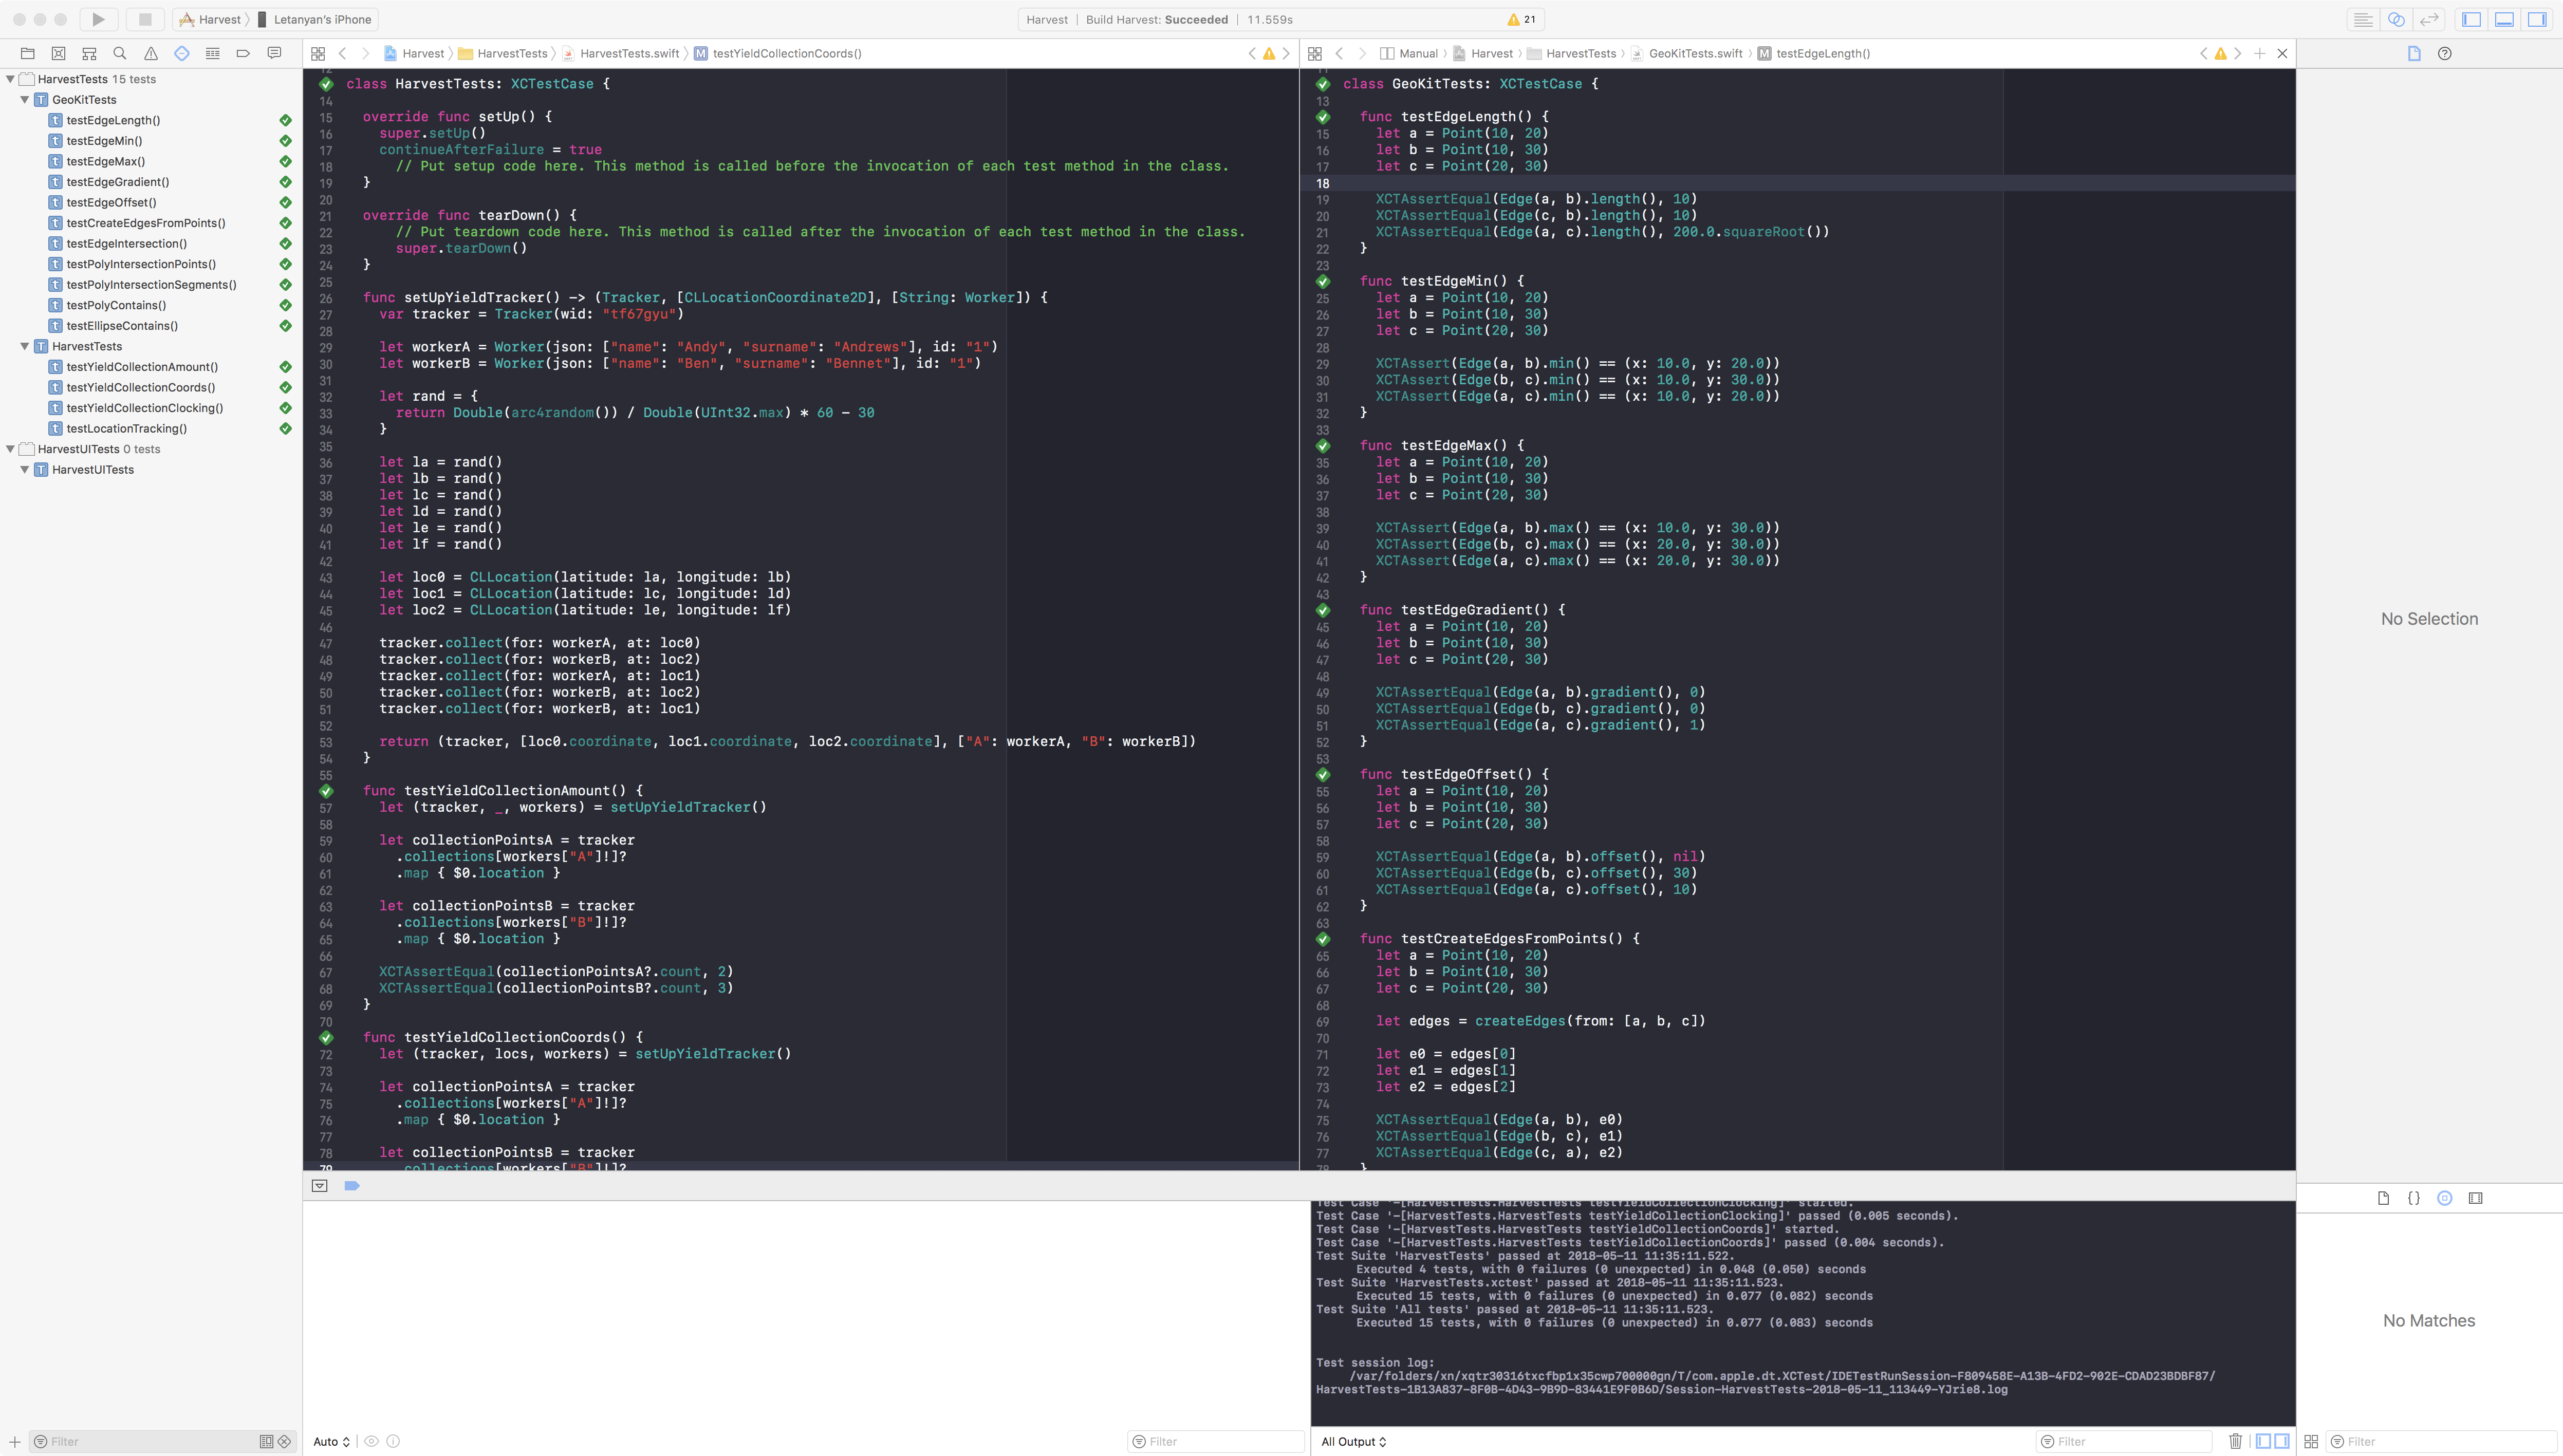
\includegraphics[width=400px]{images/iostest}
\href{https://github.com/BinaryNinjaz/COS301-Capstone/tree/master/Source/iOS/Harvest/HarvestTests}{Link to IOS App Testing}
\newline

  \subsection{NPM}
  The Ava framework will be used for automated testing purposes. To run tests one will need to run "npm test" from the testing directory.
  \subsection{XCode}
  The XCTest framework will be used for out automated testing purposes. To run tests one will need XCode. To execute the tests one will need to use XCodes build command.
 \section{TEST PROCESS}
In this section, we will illustrate a simple test process, based on IEEE-829 in order to fulfil the requirements stated in this document. \newline\newline
We can distinguish between 3 phases within the test process: \newline
\begin{enumerate}
	\item "Test specification"
	\item "Test implementation"  
	\item "Test reporting" 	
\end{enumerate}
We now intend to go through each of those 3 phases, each phase is made up of its own activities \newline
\subsection{Test specification}
The test specification can be subdivided into 2 parts. On the one hand, we have “Planning and verification”, whilst on the other, we have “Analysis, design and implementation”. \newline
Planning and verification may consist of the following activities: \newline
\begin{itemize}
 \item Specifying the scope and the risks and defining the objectives of the tests 
\item Determining the strategy
\item Taking decisions with regard to what must be tested, what roles apply, how the test activities will take place and how the outcomes of the tests will be implemented. 
\item Planning of the test design activities
\item Planning of implementation and evaluation
\end{itemize}
During the analysis, design and implementation, the test objectives will be transformed into specific test conditions and test cases. This may involve the following activities: \newline
\begin{itemize}
 \item A review of the test base (such as requirements, architecture, design, interfaces) 
\item Evaluation of the testability of the test base and the test objects 
\item Identification and prioritisation of the test conditions 
\item Designing of the test cases
\item Identifying the necessary test data in order to support the test cases 
\item Designing the test environment and identifying the infrastructure and tools 
\end{itemize}
\subsection{Implementation of tests}
The implementation of tests forms the phase in which the test procedures and scripts are implemented and the results of these (including incidents) are logged. This may involve the following activities: \newline
\begin{itemize}
 \item Implementation of the tests, manually or by means of a tool  
\item Logging the results of the implementation 
\item Comparing the results with the result that had been predicted 
\item Reporting any setbacks in the form of incidents and analysing these in order to identify the cause 
\item Repeating the tests as a result of the incidents identified 
\end{itemize}
\subsection{Test Reporting}
Test Reporting forms the phase in which the implementation of the tests is compared with the objectives. This may involve the following tasks: \newline
\begin{itemize}
 \item Checking of the test logs and the list of defects and comparing these to the exit criteria specified in the test plan   
\item Investigating whether additional tests are required
\item Writing a summary report 
\end{itemize}
  \section{TESTING PHILOSOPHY}
  Implementation of both simple and holistic tests will be of concern. However, holistic testing will be of more interest. Testing workflows are of vital importance. The project does not have many simple tasks that could provide us with the safety guarantees we would like. We instead seek to find safety in implementing tests that check the whole interaction of these few unit cases.
  
  \subsection{Benefits}
  Automated test provide developers with the ability to have safe of mind that they have not made any changes that break the program in any way or introduce bugs in any part of the program.
  Forcing developers to write tests forces them to check every part of code they write making tests a form of documentation of a projects requirements.
  
  \section{TEST EVALUATION}
  Strict zero test case failure will be followed. Any branch with a failing test case will never be merged into master. Hence we will ensure that every branch runs tests before a pull request.
  
\end{document}